\section{Evaluare}


\begin{figure}[h!]
	\centering
	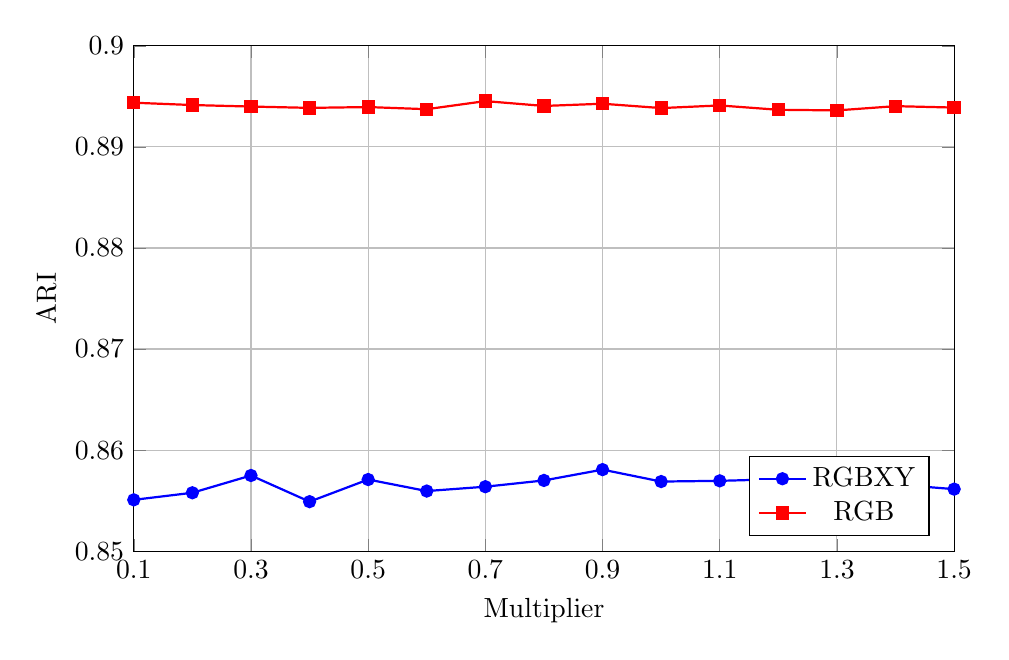
\begin{tikzpicture}
		\begin{axis}[
				width=12cm,
				height=8cm,
				xlabel={Multiplier},
				ylabel={ARI},
				xmin=0.1, xmax=1.5,
				ymin=0.85, ymax=0.90,
				xtick={0.1,0.3,0.5,0.7,0.9,1.1,1.3,1.5},
				ytick={0.85,0.86,0.87,0.88,0.89,0.90},
				legend pos=south east,
				grid=major,
			]

			\addplot[
				color=blue,
				mark=*,
				thick
			] coordinates {
					(0.1,0.85508)
					(0.2,0.85578)
					(0.3,0.85749)
					(0.4,0.85490)
					(0.5,0.85709)
					(0.6,0.85595)
					(0.7,0.85638)
					(0.8,0.85700)
					(0.9,0.85807)
					(1.0,0.85689)
					(1.1,0.85696)
					(1.2,0.85712)
					(1.3,0.85704)
					(1.4,0.85660)
					(1.5,0.85614)
				};
			\addlegendentry{RGBXY}

			\addplot[
				color=red,
				mark=square*,
				thick
			] coordinates {
					(0.1,0.89437)
					(0.2,0.89414)
					(0.3,0.89399)
					(0.4,0.89386)
					(0.5,0.89394)
					(0.6,0.89373)
					(0.7,0.89453)
					(0.8,0.89405)
					(0.9,0.89427)
					(1.0,0.89384)
					(1.1,0.89410)
					(1.2,0.89367)
					(1.3,0.89361)
					(1.4,0.89403)
					(1.5,0.89389)
				};
			\addlegendentry{RGB}

		\end{axis}
	\end{tikzpicture}
	\label{fig:ari_plot}
\end{figure}


\begin{table}[h!]
	\centering
	\begin{tabular}{|c|c|}
		\hline
		\textbf{MODEL}             & \textbf{ARI} \\
		\hline
		K-Means rgbxy              & .857         \\
		\hline
		K-Means rgb 2              & .894         \\
		\hline
		MeanshiftSegmentation      & .966         \\
		\hline
		SlotAttention Unsupervized & -.086        \\
		\hline
		SlotAttention Supervized   & -.006        \\
		\hline
		U-Net                      & .288         \\
		\hline
	\end{tabular}
	\caption{Tabel comparativ modele - ARI}
\end{table}
\section{Concluzii}
Având în vedere faptul că modelul MeanShiftSegmentation a obținut un scor considerabil de ridicat, se poate deduce
ca setul de date utilizat este relativ redus ca dimensiune si prezintă un nivel scăzut de complexitate. În mod surprinzător, modelele bazate pe tehnici de Deep Learning au înregistrat cele mai
slabe performanțe, iar arhitectura Slot Attention a obținut cele mai reduse scoruri, în ciuda faptului că a beneficiat de cele mai ample resurse de antrenare.
Performanța modelului U-Net pe datele de testare sugerează existența overfittingului.
Cu toate acestea rezultatele originale ale stiudiului ce a introdus acest mecanism\cite{locatello2020object}, duc catre posibilitate de a nu fi antrenat corect arhitectura.
Posibile viitoare rafinari includ dar nu sunt limitate la schimbarea learning rateului sau a optimizatorului. Utilizarea unui backbone deja existent. Și chiar si utilizarea unui model de difusie.
